\chapter{Extrem Value Theory distributions}
%%%%%%%%%%%%%%%%%%%%%%%%%%%%%%%%%%%%%%%%%%%%%
\section{Gumbel distribution}
\subsection{Characterization}
\begin{wrapfigure}{r}{0.5\textwidth}
  \vspace{-20pt}
  \begin{center}
    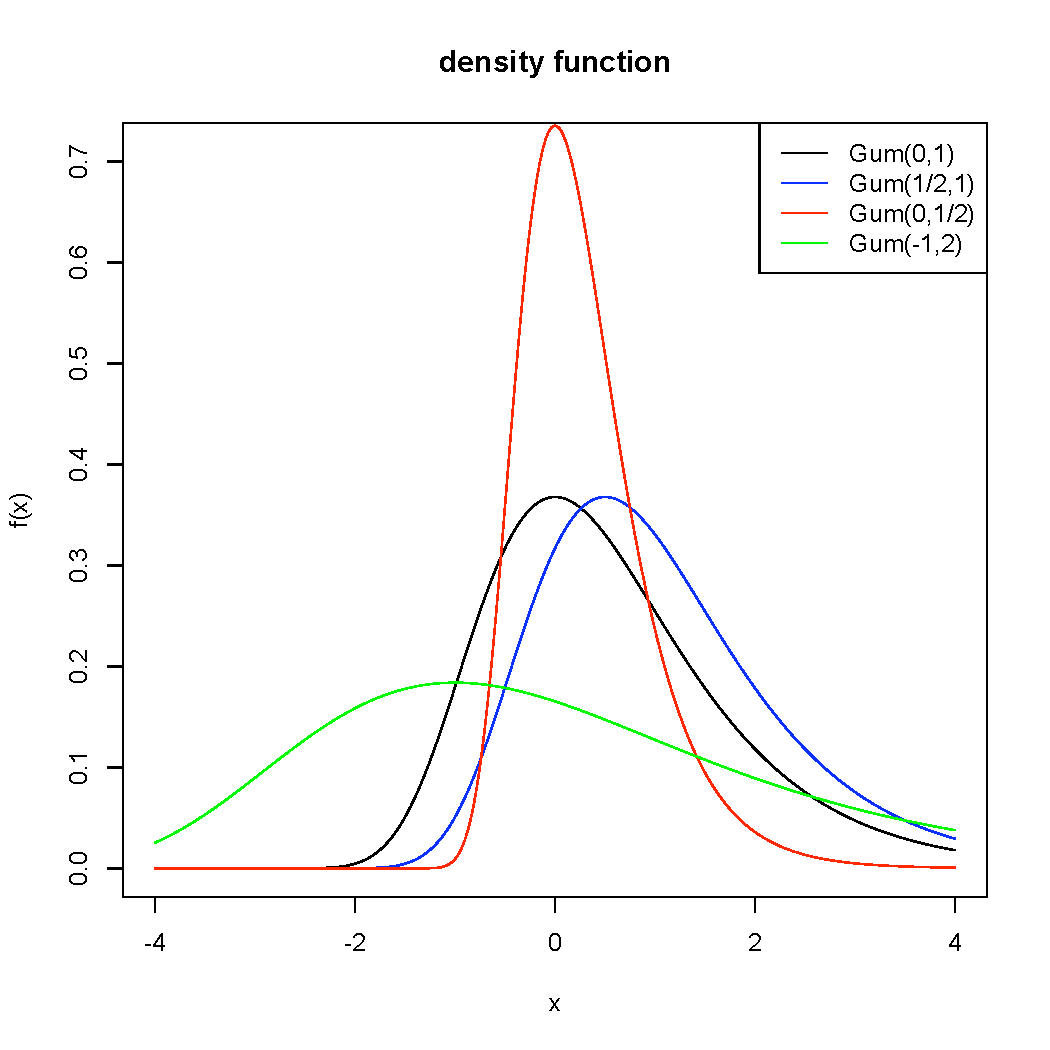
\includegraphics[width=0.48\textwidth]{img/gumbelzoom}
  \end{center}
%  \vspace{-20pt}  
  \caption{Density function for Gumbel distributions}
%  \vspace{-20pt}  
\end{wrapfigure}
The standard Gumbel distribution is defined by the following density function
$$
f(x) = e^{-x-e^{-x}},
$$
where $x\in\mathbb R$. Its distribution function is expressed as follows
$$
F(x) =e^{-e^{-x}}. 
$$

A scaled and shifted version of the Gumbel distribution exists. The density is defined as
$$
f(x)=\frac{1}{\sigma}e^{-\frac{x-\mu}{\sigma}-e^{-\frac{x-\mu}{\sigma}}},
$$
where $x\in\mathbb R$, $\mu\in\mathbb R$ and $\sigma >0$. We get back to the standard Gumbel distribution with $\mu=0$ and $\sigma=1$. The distribution function of the Gumbel I distribution is simply
$$
F(x) = e^{-e^{-\frac{x-\mu}{\sigma}}}, 
$$
for $x\in\mbb R$.

%This is the Gumbel distribution of the first kind. A completely different distribution of the Gumbel distribution can be used
%$$
%f(x) = abx^{a-1}e^{-bx^{-a}},
%$$
%where $x>0$ and $a,b>0$. The distribution function of the Gumbel II is 
%$$
%F(x) =e^{-bx^{-a}}.
%$$

There exists a Gumbel distribution of the second kind defined by the following distribution function
$$
F(x) = 1-e^{-e^{\frac{x-\mu}{\sigma}}},
$$
for $x\in\mbb R$. Hence we have the density
$$
f(x) = \frac{1}{\sigma}e^{\frac{x-\mu}{\sigma}-e^{\frac{x-\mu}{\sigma}}}.
$$
This is the distribution of $-X$ when $X$ is Gumbel I distributed.

The characteristic function of the Gumbel distribution of the first kind exists
$$
\phi(t)=\Gamma(1-i\sigma t)e^{i\mu t},
$$
while its moment generating function are
$$
M(t) = \Gamma(1-\sigma t)e^{\mu t}.
$$

\subsection{Properties}
The expectation of a Gumbel type I distribution is $E(X)=\gamma$, the Euler constant, roughly $0.57721$. Its variance is $Var(X)=\frac{\pi^2}{6}$. Thus for the Fisher-Tippett distribution, we have $E(X)=\mu+\sigma\gamma$ and $Var(X)=\frac{\pi^2\sigma^2}{6}$.

For the Gumbel type II, expectation exists if $a>1$ and variance if $a>2$.

\subsection{Estimation}
Maximum likelihood estimators are solutions of the following system
$$
\left\{
\begin{array}{l}
1=\frac{1}{n}\sum\limits_{i=1}^ne^{-\frac{X_i-\mu}{\sigma}}\\
\frac{1}{n}\sum\limits_{i=1}^n X_i=\frac{1}{n}\sum\limits_{i=1}^nX_i e^{-\frac{X_i-\mu}{\sigma}}
\end{array}
\right.,
$$
which can solved numerically initialized by the moment based estimators
$$
\tilde \mu=\bar X_n-\tilde \sigma\gamma \txtm{and} \tilde \sigma = \sqrt{\frac{6S_n^2}{\pi^2}},
$$
where $\gamma$ is the Euler constant.

\subsection{Random generation}
The quantile function of the Gumbel I distribution is simply $F^{-1}(u)=\mu-\sigma\log(-\log(u))$, thus we can use the inverse function method.

\subsection{Applications}
The Gumbel distribution is widely used in natural catastrophe modelling, especially for maximum flood.
NEED REFERENCE

%%%%%%%%%%%%%%%%%%%%%%%%%%%%%%%%%%%%%%%%%%%%%%%
\section{Fr�chet distribution}
A Fr�chet type distribution is a distribution whose distribution function is 
$$
F(x) = e^{-\left(\frac{x-\mu}{\sigma}\right)^{-\xi}},
$$
for $x\geq \mu$. One can notice this is the inverse Weibull distribution, see section \ref{invweibull} for details.


%%%%%%%%%%%%%%%%%%%%%%%%%%%%%%%%%%%%%%%%%%%%%%%%
\section{Weibull distribution}
A Weibull type distribution is characterized by the following distribution function
$$
F(x) = 1- e^{-\left(\frac{x-\mu}{\sigma}\right)^{\beta}},
$$
for $x\geq \mu$. See section \ref{weibull} for details.



%%%%%%%%%%%%%%%%%%%%%%%%%%%%%%%%%%%%%%%%%%%%%%%%
\section{Generalized extreme value distribution}
\subsection{Characterization}
The generalized extreme value distribution is defined by the following distribution function
$$
F(x)= e^{-\left(1+\xi \frac{x-\mu}{\sigma} \right)^{-\frac{1}{\xi}} },
$$
for $1+\xi\left(\frac{x-\mu}{\sigma}\right)>0$, $\xi$ the shape parameter, $\mu$ the location parameter and 
$\sigma>0$ the scale parameter. We can derive a density function
$$
f(x) =  \frac{1}{\sigma} \left(1+\xi \frac{x-\mu}{\sigma} \right)^{-\frac{1}{\xi}-1}e^{-\left(1+\xi \frac{x-\mu}{\sigma} \right)^{-\frac{1}{\xi}} }.
$$
This distribution is sometimes called the Fisher-Tippett distribution. 

Let us note that the values can be taken in $\mbb R$, $\mbb R_-$ or $\mbb R_+$ according to the sign of $\xi$. The distribution function is generally noted by $H_{\xi,\mu,\sigma}$, wich can expressed with the ``standard'' generalized extreme value distribution $H_{\xi,0,1}$ with a shift and a scaling.
When $\xi$ tends to zero, we get the Gumbel I distribution 
$$
H_{\xi,\mu,\sigma}(x) \underset{\xi\rightarrow 0}{\longrightarrow}  e^{-e^{-\frac{x-\mu}{\sigma}}}.
$$

\subsection{Properties}
The expectation and the variance are
$$
E(X) = \mu-\frac{\sigma}{\xi}\Gamma(1-\xi) \txtm{and} Var(X) = \frac{\sigma^2}{\xi^2}(\Gamma(1-2\xi)-\Gamma^2(1-\xi))
$$
if they exist.

From the extreme value theory, we have the following theorem. Let $(X_i)_{1\leq i\leq n}$ be an i.i.d. sample and $X_{i:n}$ the order statistics. If there exits two sequences $(a_n)_n$ and $(b_n)_n$ valued in 
$\mbb R_+$ and $\mbb R$ respectively, such that 
$$
P\left(\frac{X_{n:n}-b_n}{a_n}\right)
$$
have a limit in probability distribution. Then the limiting distribution $H$ for the maximum belongs to the type of one the following three distribution functions
$$
H(x)=
\left\{
\begin{array}{llr}
e^{-x^{-\xi}}, & x\geq 0, \xi>0, & \txtm{MDA of Fr�chet} \\
e^{-(-x)^{\xi}}, & x\leq 0, \xi<0, & \txtm{MDA of Weibull} \\
e^{-e^{-x}}, & x\in \mbb R, \xi=0, & \txtm{MDA of Gumbel} \\
\end{array}
\right. ,
$$
where MDA stands for maximum domains of attraction. For all distribution, there is a unique MDA. We quickly see that the limiting distribution for the maximum is nothing else than the generalized extreme value distribution $H_{\xi,0,1}$. This theorem is the Fisher-Tippett-Gnedenko theorem. 

For the minimum, assuming that $P\left(\frac{X_{1:n}-b_n}{a_n}\right)$ has a limit, the 
limiting distribution belongs to
$$
\tilde H(x)=
\left\{
\begin{array}{ll}
1-e^{-x^{\beta}}, & x\geq 0, \beta>0  \\
1-e^{-(-x)^{\beta}}, & x\leq 0, \beta<0  \\
1-e^{-e^{x}}, & x\in \mbb R, \beta=0  \\
\end{array}
\right. .
$$

In the MDA of Fr�chet, we have the Cauchy, the Pareto, the Burr, the log-gamma and the stable distributions, while in the Weibull MDA we retrieve the uniform, the beta and bounded support power law distribution. Finally, the MDA of Gumbel contains the exponential, the Weibull, the gamma, the normal, the lognormal, the Benktander distributions. 

From the \cite{tve}, we also have some equivalence given a MDA:
\begin{itemize}
\item a distribution function $F$ belongs to the MDA of Fr�chet if and only if $1- F(x)=x^{-\alpha} L(x)$ for some slowly varying function $L$,
\item a distribution function $F$ belongs to the MDA of Weibull if and only if $1- F(x_F-1/x)=x^{-\alpha} L(x)$ for some slowly varying function $L$ and $x_F<+\infty$,
\item a distribution function $F$ belongs to the MDA of Gumbel if and only if there exists $z<x_F$ such that $1- F(x)=c(x)e^{-\int_z^x\frac{g(t)}{a(t)}dt}$ for some measurable function $c$, $g$ and a continuous function $a$.
\end{itemize}

\subsection{Estimation}
According to \cite{tve} maximum likelihood estimation is not very reliable in the case of the generalized extreme value fitting. But that's not surprising since the generalized extreme value distribution is a limiting distribution to very heterogeneous distribution, such as heavy tailed, light tailed or bounded distributions.

We can use weighted moment method, where we estimate moments
$$
\omega_r(\xi,\mu,\sigma) = E(X H_{\xi,\mu,\sigma}^r(X))
$$
by its empirical equivalent
$$
\hat \omega_r = \frac{1}{n}\sum_{i=1}^n X_{j:n} U_{j:n}^r,
$$
where $U_{j:n}^r$ are the order statistics of an uniform sample (which can be replaced by its expectation $\frac{(n-r-1)!}{(n-1)!} \frac{(n-j)!}{(n-j-r)!} $).
Equalling the theoretical and the empirical moments, we get that $\xi$ is a solution of 
$$
\frac{3\hat \omega_2 -\hat\omega_0}{2\hat\omega_1-\hat\omega_0} = \frac{3^\xi-1}{2^\xi-1}.
$$
Then we estimate the other two parameters with
$$
\hat \sigma = \frac{(2\hat\omega_1-\hat\omega_0)\hat\xi}{\Gamma(1-\hat\xi)(2^{\hat\xi}-1)} \txtm{and}
\hat \mu = \hat\omega_0+\frac{\hat\sigma}{\hat\xi}(1-\Gamma(1-\hat\xi)).
$$


\subsection{Random generation}
The quantile function of the generalized extreme value distribution is 
$F^{-1}(u) = \mu+\frac{\sigma}{\xi}((-\log u)^{-\xi})-1$ for $\xi\neq 0$. So we can use the inverse function method.

\subsection{Applications}
The application of the generalized extreme value distribution is obviously the extremex value theory which can be applied in many fields : natural disaster modelling, insurance/finance extreme risk management,\dots


%%%%%%%%%%%%%%%%%%%%%%%%%%%%%%%%%%%%%%%%%%%%%%%%
\section{Generalized Pareto distribution}
See section \ref{GPD} for details.
